\chapter{Θεωρητικό Υπόβαθρο}
\label{ch:theory}

\section{Μηχανική Μάθηση και Βαθιά Μάθηση}
\label{sec:machine-deep-learning}

Η Μηχανική Μάθηση (\tl{Machine Learning}) αποτελεί κλάδο της τεχνητής
νοημοσύνης (\tl{artificial intelligence -- AI}) και περιλαμβάνει μεθόδους που επιτρέπουν στα υπολογιστικά μοντέλα
να μαθαίνουν μοτίβα και σχέσεις από δεδομένα και να τα αξιοποιούν για την
παραγωγή προβλέψεων σε νέα δεδομένα. Αυτό επιτυγχάνεται μέσω της διαδικασίας εκπαίδευσης, η οποία, ανάλογα
με τη μέθοδο, μπορεί να περιλαμβάνει την ελαχιστοποίηση μιας συνάρτησης
απώλειας (\tl{loss minimization}), τη μεγιστοποίηση της πιθανοφάνειας
(\tl{maximum likelihood estimation -- MLE}) ή την εκτίμηση της πυκνότητας
πιθανότητας (\tl{density estimation}) από τα δεδομένα
\cite{bishop2006pattern}.

Η Βαθιά Μάθηση (\tl{Deep Learning}) αποτελεί υποκατηγορία της Mηχανικής
Mάθησης και βασίζεται σε νευρωνικά δίκτυα (\tl{neural networks}) με πολλαπλά διαδοχικά επίπεδα.
Μέσω των επιπέδων αυτών, τα δίκτυα μαθαίνουν αυτόματα χαρακτηριστικά
αυξανόμενης πολυπλοκότητας \cite{goodfellow2016deep}. Στην επεξεργασία εικόνων και βίντεο, απλά
οπτικά μοτίβα συνδυάζονται στα βαθύτερα επίπεδα για την αναπαράσταση πιο
σύνθετων πληροφοριών, όπως αντικείμενα, κινήσεις και ενέργειες.

\section{Βασικές μορφές εκπαίδευσης μοντέλων Μηχανικής Μάθησης}
\label{sec:learning-paradigms}

\subsection{Επιβλεπόμενη μάθηση}
\label{subsec:supervised-learning}

Η επιβλεπόμενη μάθηση (\tl{supervised learning}) αποτελεί μία από τις πιο συνήθεις
προσεγγίσεις εκπαίδευσης Μοντέλων Μηχανικής και Βαθιάς Μάθησης.
Κατά την προσέγγιση αυτή, κάθε δείγμα του συνόλου εκπαίδευσης συνοδεύεται από μία ή περισσότερες
ετικέτες (\tl{labels}) ή τιμές-στόχους (\tl{target values}). Το μοντέλο παράγει μια πρόβλεψη για κάθε είσοδο και
μέσω μιας συνάρτησης απώλειας (\tl{loss function}) υπολογίζεται η απόκλιση της πρόβλεψης
από τον αντίστοιχο στόχο. Κατά την εκπαίδευση, οι παράμετροι του μοντέλου ενημερώνονται με σκοπό την
ελαχιστοποίηση της συνάρτησης απώλειας. Οι δύο βασικές κατηγορίες προβλημάτων επιβλεπόμενης μάθησης είναι η
ταξινόμηση (\tl{classification}), όπου ο στόχος είναι η αντιστοίχιση κάθε
δείγματος σε μία ή περισσότερες διακριτές κλάσεις από ένα προκαθορισμένο
σύνολο, και η παλινδρόμηση (\tl{regression}), όπου προβλέπονται μία ή
περισσότερες συνεχείς αριθμητικές τιμές \cite{bishop2006pattern}.

\subsection{Μη επιβλεπόμενη μάθηση}
\label{subsec:unsupervised-learning}

Στη μη επιβλεπόμενη μάθηση (\tl{unsupervised learning}), αντίθετα, τα
δεδομένα εκπαίδευσης δεν συνοδεύονται από προκαθορισμένες ετικέτες ή
τιμές-στόχους. Επομένως, το μοντέλο δεν εκπαιδεύεται με βάση γνωστές σωστές
απαντήσεις, αλλά επιδιώκει να ανακαλύψει μοτίβα, ομοιότητες και σχέσεις που
υπάρχουν στα ίδια τα δεδομένα. Στις βασικές εφαρμογές της μη επιβλεπόμενης μάθησης περιλαμβάνονται η
ομαδοποίηση (\tl{clustering}), με χαρακτηριστικό παράδειγμα τον αλγόριθμο
\tl{k-means}, και η μείωση διαστατικότητας (\tl{dimensionality reduction}),
όπως η Ανάλυση Κύριων Συνιστωσών (\tl{Principal Component Analysis -- PCA})
\cite{bishop2006pattern}, καθώς και η εκμάθηση κανόνων συσχέτισης
(\tl{association rule learning}), όπως στον αλγόριθμο \tl{Apriori}. Οι τεχνικές αυτές χρησιμοποιούνται για τη
διερευνητική ανάλυση, την προεπεξεργασία και την ανακάλυψη της εσωτερικής
δομής των δεδομένων.

\subsection{Αυτοεπιβλεπόμενη μάθηση}
\label{subsec:self-supervised-pre-training}

Η αυτοεπιβλεπόμενη μάθηση
(\tl{self-supervised learning -- SSL}) είναι μια προσέγγιση Μηχανικής
Μάθησης, που αποτελεί υποκατηγορία της μη επιβλεπόμενης μάθησης, κατά την οποία τα δεδομένα
εκπαίδευσης δεν συνοδεύονται από χειροκίνητα καθορισμένες ετικέτες ή
τιμές-στόχους. Αντίθετα, οι στόχοι εκπαίδευσης δημιουργούνται αυτόματα από
τα ίδια τα δεδομένα και το μοντέλο εκπαιδεύεται με βάση αυτούς, ώστε να
μάθει αναπαραστάσεις που περιγράφουν χρήσιμα χαρακτηριστικά και συσχετίσεις,
χωρίς να απαιτείται η χειροκίνητη επισήμανση των δεδομένων
\cite{balestriero2023cookbook}.

Κατά την εκπαίδευση με την τεχνική αυτή, επιλέγεται μια βοηθητική εργασία
(\tl{pretext task}) την οποία καλείται να επιλύσει το μοντέλο. Η εργασία
αυτή μπορεί να είναι παραγωγική (\tl{generative}), όπως η συμπλήρωση των
κρυμμένων περιοχών μιας εικόνας ή ενός βίντεο
\cite{he2022masked, wang2023videomaev2} ή η αποθορυβοποίησή τους
(\tl{denoising}) \cite{chen2025deconstructing}, ή μη παραγωγική
(\tl{non-generative}), όπως η αντιπαραθετική μάθηση (\tl{contrastive
learning}) \cite{chen2020simple}, κατά την οποία το μοντέλο μαθαίνει να
συσχετίζει διαφορετικές εκδοχές του ίδιου δείγματος οι οποίες
δημιουργούνται μέσω τεχνικών επαύξησης δεδομένων (\tl{data augmentation}),
ή η πρόβλεψη των χαρακτηριστικών (\tl{features}) που αντιστοιχούν σε
κρυμμένα τμήματα μιας εικόνας ή ενός βίντεο απευθείας στον χώρο
αναπαραστάσεων (\tl{representation space})
\cite{mahmoud2023i-jepa, adrien2023v-jepa}.

\section{Μεταφορά μάθησης}
\label{sec:transfer-learning}

Μεταφορά μάθησης (\tl{transfer learning}) ονομάζεται η διαδικασία κατά
την οποία η γνώση που αποκτά ένα μοντέλο κατά την εκπαίδευσή του για
την επίλυση μιας αρχικής εργασίας αξιοποιείται για την
επίλυση μιας νέας σχετικής εργασίας \cite{zhuang2020transfer}. Η αξιοποίηση του προεκπαιδευμένου μοντέλου
μπορεί να πραγματοποιηθεί είτε διατηρώντας τις παραμέτρους του παγωμένες,
είτε προσαρμόζοντάς τες στη νέα εργασία μέσω περαιτέρω εκπαίδευσης
(\tl{fine-tuning}).

Στην παρούσα εργασία, η βασική εφαρμογή της μεταφοράς μάθησης αφορά την
αξιοποίηση του \tl{V-JEPA Large}, το οποίο έχει προεκπαιδευτεί με
αυτοεπιβλεπόμενο τρόπο σε μια συλλογή βίντεο μεγάλης κλίμακας. Ο
προεκπαιδευμένος \tl{context encoder} διατηρείται ως παγωμένο
\tl{backbone} και επάνω στις αναπαραστάσεις του εκπαιδεύεται ένας
\tl{attentive classifier} για την αναγνώριση ανθρώπινων ενεργειών στο
\tl{HMDB51}. Επιπλέον, διερευνάται κατά πόσο η γνώση που αποκτά το 
\tl{student backbone} μέσω απόσταξης στο \tl{UCF101} μπορεί να αξιοποιηθεί
 για την επίλυση της εργασίας αναγνώρισης ανθρώπινων ενεργειών στο \tl{HMDB51}.

\section{Αναπαράσταση και κατανόηση βίντεο}
\label{sec:video-understanding}

\subsection{Ψηφιακή αναπαράσταση βίντεο}
\label{subsec:video-representation}

Μια ψηφιακή εικόνα αναπαρίσταται ως ένα δισδιάστατο πλέγμα
εικονοστοιχείων (\tl{pixels}), με ύψος \(H\) και πλάτος \(W\). Σε μια
ασπρόμαυρη εικόνα κάθε εικονοστοιχείο λαμβάνει μία τιμή φωτεινότητας,
ενώ σε μια έγχρωμη εικόνα περιγράφεται από τρεις τιμές, μία για καθένα
από τα χρωματικά κανάλια κόκκινο, πράσινο και μπλε (\tl{RGB}).
Επομένως, μια έγχρωμη εικόνα μπορεί να αναπαρασταθεί ως τανυστής
διαστάσεων \(H\times W\times C\), με \(C=3\)
\cite{tekalp2015digital}.

Προσθέτοντας σε αυτή την αναπαράσταση τη διάσταση του χρόνου, προκύπτει
το ψηφιακό βίντεο, το οποίο μπορεί να θεωρηθεί ως μια χρονικά
διατεταγμένη ακολουθία εικόνων, οι οποίες ονομάζονται καρέ
(\tl{frames}). Τα καρέ
προβάλλονται με έναν συγκεκριμένο ρυθμό (\tl{frame rate}), ο οποίος
εκφράζει το πλήθος των καρέ ανά δευτερόλεπτο και μετράται σε
\tl{frames per second -- FPS} \cite{tekalp2015digital}. Για ένα βίντεο διάρκειας \(\tau\) δευτερολέπτων και σταθερού ρυθμού
\(f\) καρέ ανά δευτερόλεπτο, το πλήθος των καρέ \(T\) δίνεται
προσεγγιστικά από τη σχέση:

\begin{equation}
    T \approx \tau \cdot f.
\end{equation}

Καθώς κάθε καρέ αποτελεί μια έγχρωμη εικόνα διαστάσεων
\(H \times W \times C\), ένα απόσπασμα βίντεο με \(T\) καρέ μπορεί να
αναπαρασταθεί ως τανυστής \cite{arnab2021vivit}:

\begin{equation}
    \mathbf{V} \in \mathbb{R}^{T \times H \times W \times C}.
\end{equation}

Τα βίντεο μπορεί να έχουν διαφορετική διάρκεια και να περιλαμβάνουν μεγάλο
αριθμό καρέ. Για τον λόγο αυτό, τα μοντέλα κατανόησης βίντεο συνήθως δεν
επεξεργάζονται ολόκληρο το αρχικό βίντεο, αλλά αποσπάσματα
(\tl{video clips}) τα οποία περιέχουν έναν προκαθορισμένο αριθμό καρέ. Η
επιλογή των καρέ πραγματοποιείται μέσω χρονικής δειγματοληψίας
(\tl{temporal sampling}). Ανάλογα με την εφαρμογή, τα καρέ μπορεί να δειγματοληπτούνται διαδοχικά, ομοιόμορφα
σε όλη τη διάρκεια του βίντεο, τυχαία ή με συγκεκριμένο χρονικό βήμα
(\tl{sampling stride}). Με αυτόν τον τρόπο 
παράγονται είσοδοι σταθερών διαστάσεων, οι οποίες μπορούν να επεξεργαστούν
από τα μοντέλα κατανόησης βίντεο.

\subsection{Αναγνώριση ανθρώπινων ενεργειών}
\label{subsec:human-action-recognition}

Η αναγνώριση ανθρώπινων ενεργειών (\tl{human action recognition}) αποτελεί 
μία από τις σημαντικότερες εργασίες κατανόησης βίντεο στην υπολογιστική όραση (\tl{computer vision}). 
Στόχος της είναι η αυτόματη ανάλυση ενός βίντεο εισόδου και η ταξινόμηση της 
ανθρώπινης ενέργειας που απεικονίζεται σε αυτό. Για την εκπαίδευση και την αξιολόγηση 
μοντέλων στην εργασία αυτή έχουν χρησιμοποιθεί και επεξεργαστεί δύο επισημασμένα σύνολα δεδομένων, 
το \tl{HMDB51}\cite{kuehne2011hmdb} και το \tl{UCF101}\cite{soomro2012ucf101}, τα βίντεο των οποίων προέρχονται από καταγραφές, ταινίες, τηλεοπτικό υλικό και 
διαδικτυακές πλατφόρμες.

Η αναγνώριση ανθρώπινων ενεργειών αποτελεί ένα απαιτητικό πρόβλημα, καθώς η
ίδια ενέργεια μπορεί να εκτελείται με διαφορετικό τρόπο, ταχύτητα ή διάρκεια
από διαφορετικά άτομα. Πρόσθετες δυσκολίες προκύπτουν από τις αλλαγές στην
οπτική γωνία και στον φωτισμό, την κίνηση της κάμερας, το σύνθετο ή
μεταβαλλόμενο φόντο και τη μερική απόκρυψη του ανθρώπινου σώματος από άλλα
αντικείμενα \cite{jegham2020vision}. Παράλληλα, διαφορετικές ενέργειες
μπορεί να μοιάζουν σε μεμονωμένα καρέ. Για τον
λόγο αυτό, η αποτελεσματική αναγνώρισή τους απαιτεί την αξιοποίηση τόσο της
χωρικής πληροφορίας κάθε καρέ όσο και της χρονικής μεταβολής μεταξύ
διαδοχικών καρέ.
\section{\tl{Transformer} και \tl{Vision Transformer}}
\label{sec:transformer-vision-transformer}

\subsection{O \tl{Transformer}}
\label{subsec:transformer}

O \tl{Transformer} παρουσιάστηκε για πρώτη φορά στην εργασία
\tl{Attention Is All You Need} \cite{vaswani2017attention}, με σκοπό την
επεξεργασία ακολουθιών χωρίς τη χρήση αναδρομικών ή συνελικτικών νευρωνικών
δικτύων. Αποτέλεσε σημαντικό ορόσημο στην εξέλιξη της Βαθιάς Μάθησης και
αποτελεί τη βάση πολλών σύγχρονων αρχιτεκτονικών, όπως τα μεγάλα γλωσσικά
μοντέλα (\tl{Large Language Models -- LLMs}), τα μοντέλα κατανόησης εικόνας και
βίντεο και τα μοντέλα όρασης και γλώσσας (\tl{Vision-Language Models -- VLMs}).

Η αρχιτεκτονική  του \tl{Transformer} αποτελείται από έναν
κωδικοποιητή (\tl{encoder}) και έναν αποκωδικοποιητή (\tl{decoder}). Ο 
κωδικοποιητής επεξεργάζεται την ακολουθία εισόδου και δημιουργεί μια
αναπαράστασή της. Σε κάθε βήμα, ο αποκωδικοποιητής συνδυάζει την
αναπαράσταση αυτή με τα στοιχεία της εξόδου που έχει ήδη παράγει, ώστε να
προβλέψει το επόμενο στοιχείο.

Ο κωδικοποιητής και ο αποκωδικοποιητής αποτελούνται από διαδοχικά
\tl{Transformer blocks}, στα οποία βασικό στοιχείο είναι ο μηχανισμός
\tl{multi-head attention}.

\subsection{Μηχανισμός αυτοπροσοχής}
\label{subsec:self-attention}

Ο μηχανισμός προσοχής (\tl{attention}) επιτρέπει σε ένα μοντέλο να αποδίδει
διαφορετικό βαθμό σημασίας στα επιμέρους στοιχεία της εισόδου κατά την
επεξεργασία της. Η αυτοπροσοχή (\tl{self-attention}), στην οποία βασίζεται ο \tl{Transformer}, αποτελεί ειδική περίπτωση
του μηχανισμού προσοχής, κατά την οποία κάθε στοιχείο της εισόδου
αλληλεπιδρά με όλα τα υπόλοιπα στοιχεία της ίδιας ακολουθίας. Με αυτόν τον
τρόπο, το μοντέλο μπορεί να μάθει σχέσεις και εξαρτήσεις μεταξύ στοιχείων που
βρίσκονται σε διαφορετικές θέσεις της εισόδου.

Για τον υπολογισμό της αυτοπροσοχής, η είσοδος \(X\) προβάλλεται αρχικά στους
πίνακες ερωτημάτων (\tl{queries}) \(Q\), κλειδιών (\tl{keys}) \(K\) και τιμών
(\tl{values}) \(V\), σύμφωνα με τις σχέσεις:

\begin{equation}
    Q=XW_Q,\qquad K=XW_K,\qquad V=XW_V,
\end{equation}

όπου \(W_Q\), \(W_K\) και \(W_V\) είναι εκπαιδεύσιμοι πίνακες βαρών. Στη
συνέχεια, η κλιμακωμένη προσοχή εσωτερικού γινομένου
(\tl{scaled dot-product attention}) υπολογίζεται ως

\begin{equation}
    \operatorname{Attention}(Q,K,V)
    =
    \operatorname{softmax}
    \left(
        \frac{QK^{\top}}{\sqrt{d_k}}
    \right)V,
    \label{eq:attention}
\end{equation}

όπου \(d_k\) είναι η διάσταση κάθε διανύσματος του πίνακα \(K\). Το γινόμενο
\(QK^{\top}\) υπολογίζει τον βαθμό συσχέτισης μεταξύ των στοιχείων της
εισόδου, ενώ η συνάρτηση \tl{softmax} μετατρέπει τις τιμές αυτές σε βάρη
προσοχής. Τα βάρη εφαρμόζονται στις τιμές \(V\), ώστε να παραχθεί η τελική
έξοδος του μηχανισμού \cite{vaswani2017attention}.

Για ένα διάνυσμα \(z=(z_1,\ldots,z_n)\), η συνάρτηση \tl{softmax} ορίζεται ως

\begin{equation}
    \operatorname{softmax}(z)_i
    =
    \frac{e^{z_i}}{\sum_{j=1}^{n}e^{z_j}},
    \qquad i=1,\ldots,n.
    \label{eq:softmax}
\end{equation}

Η συνάρτηση \tl{softmax} μετατρέπει τις αρχικές τιμές σε αριθμούς μεταξύ
μηδέν και ένα, των οποίων το άθροισμα ισούται με τη μονάδα. Οι αριθμοί αυτοί
σχηματίζουν μια κατανομή πιθανότητας και εκφράζουν τη σχετική σημασία κάθε
στοιχείου. Επομένως, μεγαλύτερη τιμή συσχέτισης στο \(QK^{\top}\) οδηγεί σε
μεγαλύτερο βάρος προσοχής για το αντίστοιχο στοιχείο της εισόδου.

Το \tl{multi-head attention} αποτελεί επέκταση του παραπάνω μηχανισμού, στην
οποία εφαρμόζονται παράλληλα \(h\) διαφορετικές κεφαλές προσοχής. Όλες οι
κεφαλές λαμβάνουν ολόκληρη την ακολουθία εισόδου, αλλά καθεμία την προβάλλει
σε διαφορετικό, συνήθως μικρότερης διάστασης, υποχώρο χαρακτηριστικών μέσω
διαφορετικών εκπαιδεύσιμων πινάκων βαρών. Η έξοδος της κεφαλής \(i\) δίνεται
από τη σχέση

\begin{equation}
    \operatorname{head}_i
    =
    \operatorname{Attention}
    \left(XW_i^Q, XW_i^K, XW_i^V\right),
    \label{eq:attention-head}
\end{equation}

ενώ οι έξοδοι όλων των κεφαλών συνενώνονται (\tl{concatenation}) και
προβάλλονται μέσω του πίνακα \(W^O\):

\begin{equation}
    \operatorname{MultiHead}(X)
    =
    \operatorname{Concat}
    \left(\operatorname{head}_1,\ldots,\operatorname{head}_h\right)W^O.
    \label{eq:multi-head-attention}
\end{equation}

Οι πίνακες προβολής έχουν διαστάσεις
\(W_i^Q \in \mathbb{R}^{d_{\mathrm{model}}\times d_k}\),
\(W_i^K \in \mathbb{R}^{d_{\mathrm{model}}\times d_k}\),
\(W_i^V \in \mathbb{R}^{d_{\mathrm{model}}\times d_v}\) και
\(W^O \in \mathbb{R}^{h d_v\times d_{\mathrm{model}}}\), όπου
\(d_{\mathrm{model}}\) είναι η διάσταση της αναπαράστασης εισόδου, \(d_v\) η
διάσταση των τιμών και \(h\) το πλήθος των κεφαλών
\ref{fig:multihead-attention}.

Με αυτόν τον τρόπο, κάθε κεφαλή μπορεί να εστιάζει σε διαφορετικές σχέσεις
μεταξύ των στοιχείων της ίδιας εισόδου. Η συνένωση των επιμέρους εξόδων
επιτρέπει στο μοντέλο να συνδυάζει ταυτόχρονα αυτές τις διαφορετικές
συσχετίσεις σε μία ενιαία αναπαράσταση.

\begin{figure}[H]
    \centering
    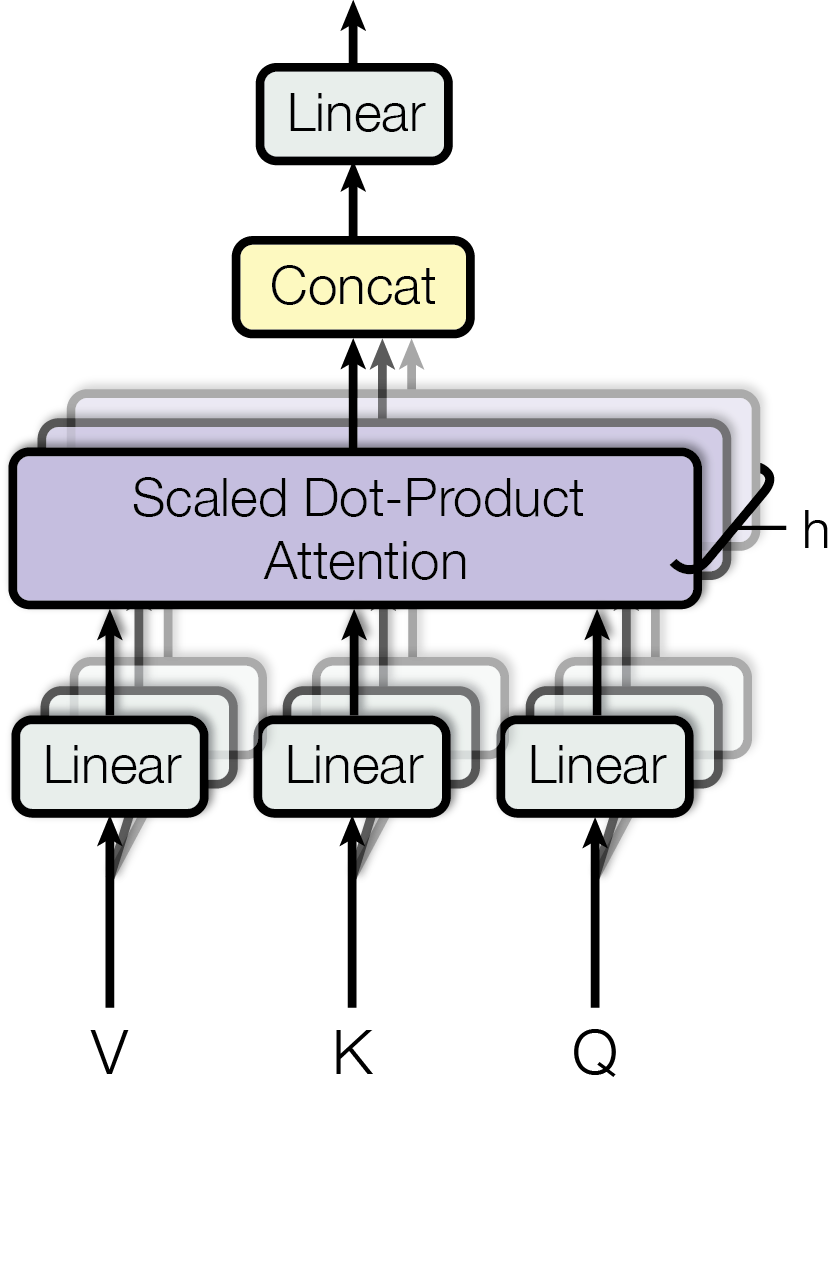
\includegraphics[width=0.45\textwidth]{ModalNet-20.png}
    \caption{Ο μηχανισμός \tl{multi-head attention}. Πηγή:
    \cite{vaswani2017attention}.}
    \label{fig:multihead-attention}
\end{figure}


\subsection{\tl{Vision Transformers} για εικόνες και βίντεο}
\label{subsec:vit-architecture}

Ο \tl{Vision Transformer -- ViT} προτάθηκε στην εργασία \tl{"An Image is Worth 16x16 Words: Transformers for Image Recognition at Scale"}
\cite{dosovitskiy2021image} ως μια εναλλακτική προσέγγιση των συνελικτικών
νευρωνικών δικτύων (\tl{CNNs}) για την επεξεργασία εικόνων. Στη συνέχεια, η βασική του
αρχιτεκτονική επεκτάθηκε και στην επεξεργασία βίντεο στην εργασία \tl{"Video Vision Transformer -- ViViT: A Video Vision Transformer"} \cite{arnab2021vivit}.

\begin{figure}[H]
    \centering
    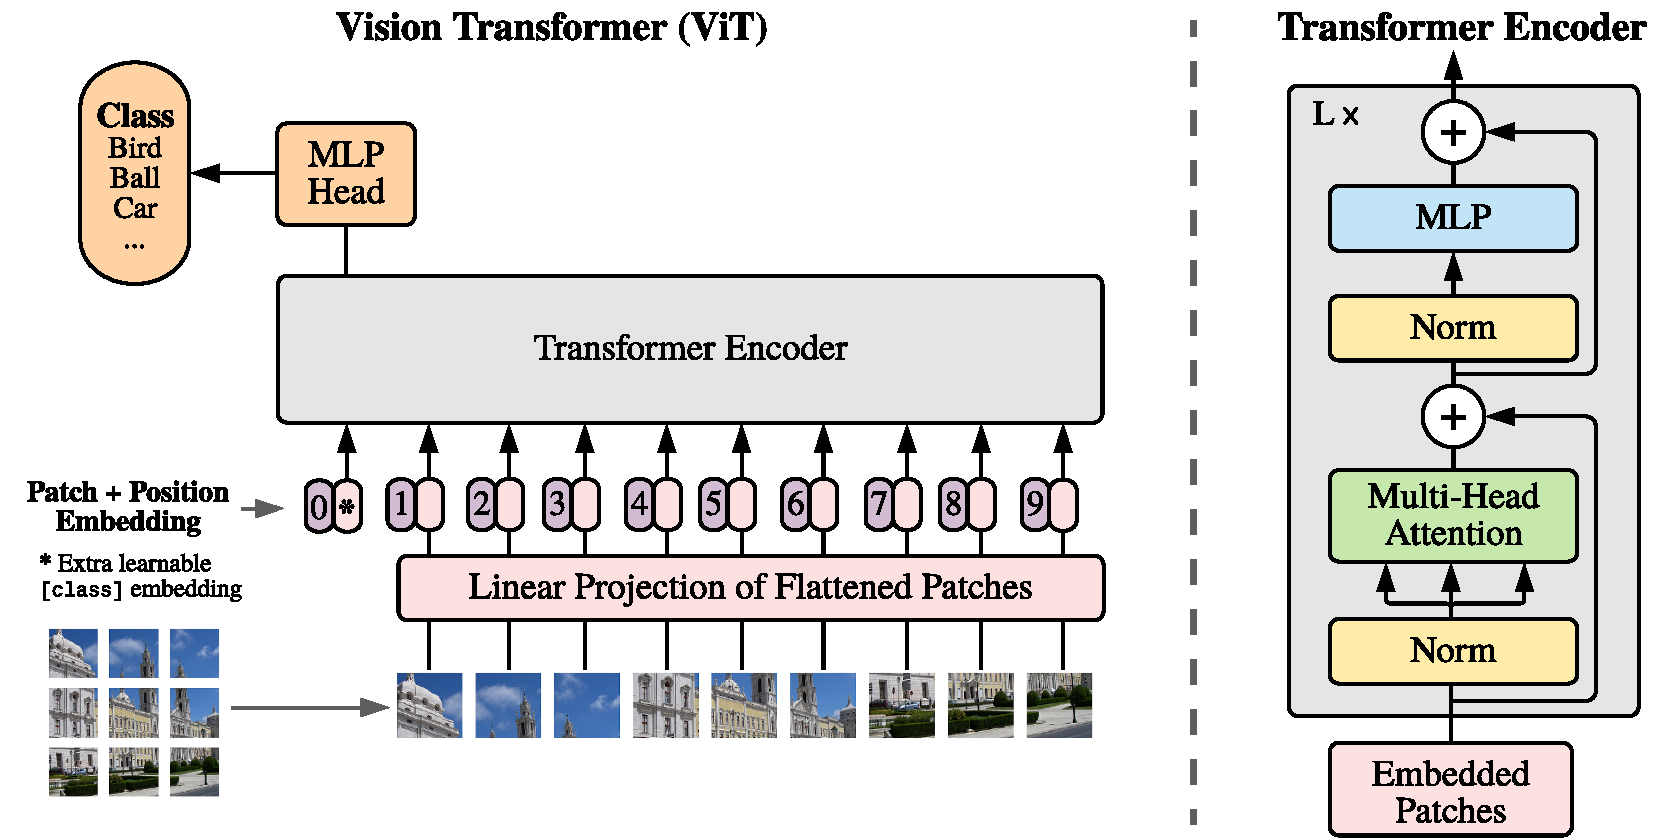
\includegraphics[width=\textwidth]{model_scheme.pdf}
    \caption{Η αρχιτεκτονική του \tl{Vision Transformer (ViT)}. Πηγή:
    \cite{dosovitskiy2021image}.}
    \label{fig:vit-architecture}
\end{figure}

Ο \tl{ViT} αποτελείται από έναν κωδικοποιητή \tl{Transformer}, ο οποίος
δέχεται ως είσοδο μια ακολουθία από \tl{tokens}. Για τη δημιουργία τους, η
δισδιάστατη εικόνα χωρίζεται σε μη επικαλυπτόμενα τμήματα σταθερού μεγέθους
(\tl{patches}). Έστω μια εικόνα
\(\mathbf{x}\in\mathbb{R}^{H\times W\times C}\), η οποία χωρίζεται σε
τετραγωνικά \tl{patches} μεγέθους \(P\times P\). Το πλήθος τους δίνεται από:

\begin{equation}
    N=\frac{HW}{P^2}.
    \label{eq:number-image-patches}
\end{equation}

Κάθε \tl{patch} αποτελείται από τις τιμές των \tl{pixels} για καθένα από τα
χρωματικά κανάλια της αντίστοιχης περιοχής της εικόνας. Οι τιμές αυτές τοποθετούνται διαδοχικά σε ένα διάνυσμα μέσω της
διαδικασίας \tl{flattening}. Επομένως, το σύνολο των \tl{patches}
αναπαρίσταται ως:

\begin{equation}
    \mathbf{x}_p\in\mathbb{R}^{N\times(P^2C)}.
    \label{eq:flattened-image-patches}
\end{equation}

Στη συνέχεια, ένας εκπαιδεύσιμος πίνακας
\(\mathbf{E}\in\mathbb{R}^{P^2C\times D}\) προβάλλει γραμμικά κάθε
διάνυσμα σε ένα \tl{token} διάστασης \(D\), το οποίο αποτελεί την
αναπαράσταση του αντίστοιχου \tl{patch}.

Στην ακολουθία προστίθεται ένα εκπαιδεύσιμο \tl{class token}, του οποίου η
τελική αναπαράσταση χρησιμοποιείται για την ταξινόμηση της εικόνας. Επιπλέον,
στα \tl{tokens} προστίθενται εκπαιδεύσιμες κωδικοποιήσεις θέσης
(\tl{learnable positional embeddings}), ώστε το μοντέλο να διατηρεί
πληροφορίες σχετικά με τη χωρική θέση κάθε \tl{patch} στην αρχική εικόνα. Η
αρχική ακολουθία εισόδου του κωδικοποιητή γράφεται ως:

\begin{equation}
    \mathbf{z}_0=
    \left[
        \mathbf{x}_{\mathrm{class}};
        \mathbf{x}_p^1\mathbf{E};
        \mathbf{x}_p^2\mathbf{E};
        \ldots;
        \mathbf{x}_p^N\mathbf{E}
    \right]
    +\mathbf{E}_{\mathrm{pos}},
    \label{eq:vit-input-sequence}
\end{equation}

όπου \(\mathbf{x}_{\mathrm{class}}\) είναι το εκπαιδεύσιμο \tl{class token}
και \(\mathbf{E}_{\mathrm{pos}}\in\mathbb{R}^{(N+1)\times D}\) οι
κωδικοποιήσεις θέσης.

Στην περίπτωση ενός βίντεο
\(\mathbf{V}\in\mathbb{R}^{T\times H\times W\times C}\), η διαδικασία
είναι παρόμοια, με τη διαφορά ότι η είσοδος χωρίζεται σε τρισδιάστατα
χωροχρονικά τμήματα
(\tl{tubelets}). Κάθε \tl{tubelet} καλύπτει μια συγκεκριμένη χωρική περιοχή
μεγέθους \(P\times P\) σε \(P_t\) διαδοχικά καρέ. Το συνολικό πλήθος των
\tl{tubelets} είναι:

\begin{equation}
    N_v=
    \frac{T}{P_t}\frac{H}{P}\frac{W}{P}.
    \label{eq:number-video-tokens}
\end{equation}

Οι \(P_tP^2C\) τιμές κάθε \tl{tubelet} μετατρέπονται σε διάνυσμα μέσω
\tl{flattening} και στη συνέχεια προβάλλονται γραμμικά σε ένα χωροχρονικό
\tl{token} διάστασης \(D\). Επομένως, το βίντεο αναπαρίσταται ως ακολουθία:

\begin{equation}
    \widetilde{\mathbf{z}}\in\mathbb{R}^{N_v\times D}.
    \label{eq:video-token-sequence}
\end{equation}

Με αυτόν τον τρόπο, η ακολουθία εισόδου περιλαμβάνει πληροφορίες τόσο για το
περιεχόμενο των καρέ όσο και για τη χρονική εξέλιξη του βίντεο.

Τόσο στην περίπτωση των εικόνων όσο και στην περίπτωση των βίντεο, ο
\tl{ViT} αποτελείται από \(L\) διαδοχικά \tl{Transformer blocks}. Η
έξοδος κάθε \tl{block} χρησιμοποιείται ως είσοδος στο επόμενο. 
Κάθε \tl{ViT block} επεξεργάζεται την ακολουθία των \tl{tokens} σε
δύο διαδοχικά στάδια. Αρχικά, η είσοδος περνά από ένα επίπεδο \tl{Layer Normalization} και στη συνέχεια από
τον μηχανισμό \tl{multi-head self-attention}. Η έξοδος του μηχανισμού
προστίθεται στην αρχική είσοδο μέσω ενός \tl{residual connection}. Η
αναπαράσταση που προκύπτει περνά από ένα δεύτερο επίπεδο
\tl{Layer Normalization} και από ένα \tl{MLP block}, του οποίου η έξοδος
προστίθεται ξανά στην είσοδο του συγκεκριμένου σταδίου. Η διαδικασία αυτή για
το επίπεδο \(\ell\) περιγράφεται από τις σχέσεις:

\begin{equation}
    \mathbf{y}^{\ell}
    =
    \operatorname{MSA}
    \left(
        \operatorname{LN}(\mathbf{z}^{\ell-1})
    \right)
    +
    \mathbf{z}^{\ell-1},
    \label{eq:vit-msa-block}
\end{equation}

\begin{equation}
    \mathbf{z}^{\ell}
    =
    \operatorname{MLP}
    \left(
        \operatorname{LN}(\mathbf{y}^{\ell})
    \right)
    +
    \mathbf{y}^{\ell},
    \label{eq:vit-mlp-block}
\end{equation}

όπου \tl{MSA} είναι ο μηχανισμός \tl{multi-head self-attention} και \tl{LN}
το επίπεδο \tl{Layer Normalization}. Στην κλασική αρχιτεκτονική
ταξινόμησης του \tl{ViT}, μετά την επεξεργασία από όλα τα
\tl{Transformer blocks}, η τελική αναπαράσταση του \tl{class token} δίνεται
ως είσοδος σε μια κεφαλή ταξινόμησης (\tl{classification head}), η οποία
παράγει τις προβλέψεις για τις διαφορετικές κατηγορίες \ref{fig:vit-architecture}.

\section{Το μοντέλο \tl{V-JEPA}}
\label{sec:vjepa}

\subsection{Η αφετηρία, το μοντέλο \tl{I-JEPA}}
\label{sec:ijepa}

Το \tl{I-JEPA} που παρουσιάστηκε στην εργασία \tl{Self-Supervised Learning
from Images with a Joint-Embedding Predictive Architecture}
\cite{mahmoud2023i-jepa}, αποτέλεσε μια μη παραγωγική μέθοδο
αυτοεπιβλεπόμενης μάθησης για την εκμάθηση αναπαραστάσεων από εικόνες. Η αρχιτεκτονική
\tl{Joint-Embedding Predictive Architecture} που χρησιμοποιεί αποτελείται
από έναν \tl{context encoder} (\tl{x-encoder}), έναν \tl{target encoder}
(\tl{y-encoder}) και έναν \tl{predictor}, που βασίζονται στους \tl{Vision
Transformers}. Χρησιμοποιώντας την τεχνική απόκρυψης (\tl{masking}), το
μοντέλο προεκπαιδεύεται ώστε ο \tl{predictor}, με βάση την αναπαράσταση
που παρήγαγε ο \tl{context encoder}, να προβλέπει τις αναπαραστάσεις
κρυμμένων περιοχών της εικόνας $\hat{s}_y$, όπως αυτές υπολογίζονται από
τον \tl{target encoder} στον χώρο των αναπαραστάσεων (\tl{feature space})
$s_y$ /ref{fig:ijepa-architecture}.

\vspace{0.5cm}
\begin{figure}[ht]
    \centering
    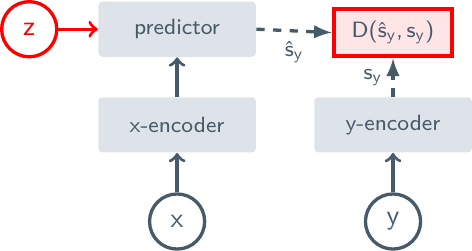
\includegraphics[width=0.6\textwidth]{fig2_jepa-1.png}
    \caption{Αρχιτεκτονική \tl{JEPA}.
    Πηγή: \cite{adrien2023v-jepa}.}
    \label{fig:ijepa-architecture}
\end{figure}

\subsection{Βασική ιδέα του \tl{V-JEPA}}
\label{subsec:vjepa-overview}

Το \tl{V-JEPA}\cite{adrien2023v-jepa} αποτελεί επέκταση του \tl{I-JEPA} από τις εικόνες στα
δεδομένα βίντεο, βασιζόμενο στην ίδια αρχιτεκτονική \tl{JEPA}. Η βασική
ιδέα του παραμένει η αξιοποίηση της πρόβλεψης στον χώρο των αναπαραστάσεων
ως στόχου αυτοεπιβλεπόμενης εκπαίδευσης (\tl{SSL objective}) για δεδομένα
βίντεο. Με αυτή τη μη παραγωγική προσέγγιση,
το μοντέλο μαθαίνει χρήσιμα και γενικεύσιμα χαρακτηριστικά, χωρίς να
απαιτεί τη χρήση προεκπαιδευμένου κωδικοποιητή εικόνων, αρνητικών
δειγμάτων ή δαπανηρής ανακατασκευής \tl{pixels}. Καθίσταται έτσι ικανό να
αξιοποιηθεί σε διαφορετικές εργασίες εικόνας και βίντεο, αποτελώντας ένα
\tl{video foundation model}.

\subsection{Διαδικασία προεκπαίδευσης του \tl{V-JEPA}}
\label{subsec:vjepa-pretraining}

Για την προεκπαίδευση του \tl{V-JEPA} χρησιμοποιήθηκε το \tl{VideoMix2M},
ένα σύνολο περίπου δύο εκατομμυρίων βίντεο που προέκυψε από τον
συνδυασμό διαφόρων δημόσιων συνόλων βίντεο. Η ίδια αρχή πρόβλεψης
αναπαραστάσεων που περιγράφηκε παραπάνω για το \tl{I-JEPA} εφαρμόζεται
και εδώ, προσαρμοσμένη στη χωροχρονική φύση των δεδομένων βίντεο.

\begin{figure}[H]
    \centering
    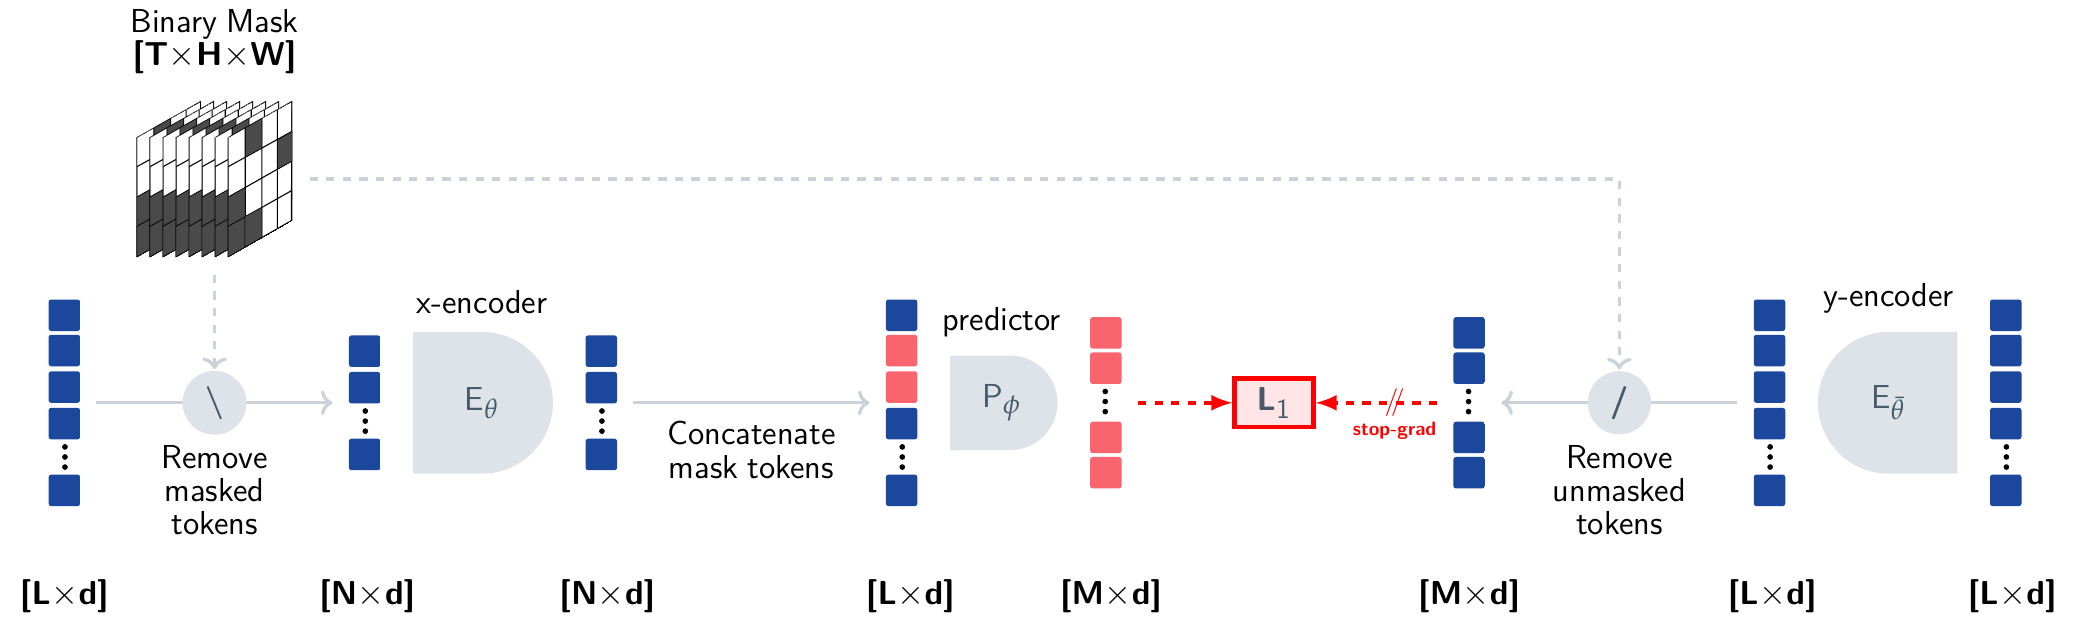
\includegraphics[width=\textwidth]{fig3_vjepa_complex-1.png}
    \caption{Αρχιτεκτονική και διαδικασία προεκπαίδευσης του \tl{V-JEPA}.
    Πηγή: \cite{adrien2023v-jepa}.}
    \label{fig:vjepa-architecture}
\end{figure}

Κατά την προεκπαίδευση, από κάθε βίντεο επιλέγεται ένα απόσπασμα 16 καρέ,
το οποίο μετατρέπεται σε μια ακολουθία από \tl{tubelet tokens}. Καθένα από
αυτά αντιστοιχεί σε ένα χωροχρονικό τμήμα που εκτείνεται σε δύο διαδοχικά
καρέ. Τα \tl{tokens} τροφοδοτούνται στον \tl{target encoder}, ο οποίος
παράγει τις αναπαραστάσεις τους. Στη συνέχεια, μέσω τυχαίας δειγματοληψίας
δημιουργούνται χωροχρονικές μάσκες, οι οποίες εκτείνονται σε όλα τα καρέ
του αποσπάσματος. Με βάση τις μάσκες αυτές επιλέγονται από την έξοδο του
\tl{target encoder} οι αναπαραστάσεις που θα χρησιμοποιηθούν ως στόχοι
πρόβλεψης.

Οι ίδιες μάσκες εφαρμόζονται στην είσοδο του \tl{context encoder}, ώστε
αυτός να επεξεργάζεται μόνο τα μη αποκρυμμένα \tl{tokens}. Οι
αναπαραστάσεις που παράγει δίνονται ως είσοδος στον \tl{predictor} μαζί
με εκπαιδεύσιμα \tl{mask tokens}, στα οποία προστίθονται επίσης \tl{positional embeddings} για τη θέση των
αποκρυμμένων περιοχών. Με βάση τον συνδυασμό των δύο, ο \tl{predictor}
παράγει προβλέψεις για τις αντίστοιχες αναπαραστάσεις-στόχους \ref{fig:vjepa-architecture}.

Η εκπαίδευση πραγματοποιείται ελαχιστοποιώντας, μέσω της νόρμας
$\ell_1$, την απόκλιση μεταξύ των αναπαραστάσεων που προβλέπει ο
\tl{predictor} και των αντίστοιχων αναπαραστάσεων που παράγει ο
\tl{target encoder}:
\begin{equation}
    \min_{\theta,\phi} \left\| P_\phi\big(E_\theta(x), \Delta y\big)
    - \operatorname{sg}\big(E_{\bar\theta}(y)\big) \right\|_1
\end{equation}
Στις αναπαραστάσεις του \tl{target encoder} εφαρμόζεται \tl{stop-gradient}
($\operatorname{sg}$), ώστε οι παράμετροί του να μην ενημερώνονται κατά το
\tl{backpropagation}. Αντ' αυτού, ενημερώνονται μέσω εκθετικού κινητού
μέσου (\tl{Exponential Moving Average}) των παραμέτρων του \tl{context
encoder}: σε κάθε βήμα εκπαίδευσης, τα βάρη $\bar\theta$ του \tl{target
encoder} ενημερώνονται ως:
\begin{equation}  
    \bar\theta \leftarrow \tau \bar\theta + (1 - \tau)\theta
\end{equation}
όπου $\theta$ τα βάρη του \tl{context encoder} και $\tau \in (0,1)$ μια
παράμετρος \tl{momentum}. Σύμφωνα με τους συγγραφείς, η χρήση του
εκθετικού κινητού μέσου για τον υπολογισμό των αναπαραστάσεων-στόχων
διασφαλίζει ότι ο \tl{predictor} εξελίσσεται ταχύτερα από τον \tl{target
encoder} και παραμένει κοντά στη βέλτιστη λύση, αποτρέποντας έτσι το
φαινόμενο της κατάρρευσης αναπαραστάσεων (\tl{representation collapse})
\cite{adrien2023v-jepa}.

Τελικός στόχος της προεκπαίδευσης είναι ο \tl{context encoder} να μάθει
να παράγει γενικεύσιμες και πλούσιες σε πληροφορία αναπαραστάσεις για τις εικόνες ή βίντεο που του δίνονται ως είσοδος. Με την
ολοκλήρωση της προεκπαίδευσης, διατηρείται αποκλειστικά ο \tl{context
encoder}, ο οποίος χρησιμοποιείται ως \tl{backbone} για την εξαγωγή
αναπαραστάσεων από νέα δεδομένα βίντεο. Αντίθετα, ο \tl{target encoder}
και ο \tl{predictor} χρησιμοποιούνται μόνο κατά την προεκπαίδευση και δεν
συμμετέχουν σε καμία άλλη εργασία.

\subsection{Παραλλαγές μεγέθους του \tl{V-JEPA}}
\label{subsec:vjepa-model-sizes}

Για την αξιοποίηση του \tl{context encoder} ως εξαγωγέα χαρακτηριστικών (\tl{feature extractor}), η
αρχιτεκτονική του μπορεί να διαμορφωθεί σε διαφορετικά μεγέθη. Στην παρούσα
εργασία χρησιμοποιούνται οι παραλλαγές \tl{Large}, \tl{Base}, \tl{Small} και
\tl{Tiny}. Οι αρχιτεκτονικές αυτές διαφέρουν ως προς τη διάσταση των
αναπαραστάσεων, τον αριθμό των \tl{Transformer blocks}, τον αριθμό των
\tl{attention heads} και τον συνολικό αριθμό των παραμέτρων τους. Ο
Πίνακας~\ref{tab:vjepa-model-sizes} συνοψίζει τα βασικά χαρακτηριστικά τους.

\begin{table}[H]
    \centering
    \small
    \setlength{\tabcolsep}{5pt}
    \caption{Χαρακτηριστικά των \tl{V-JEPA backbones}.}
    \label{tab:vjepa-model-sizes}
    \begin{tabular}{lccccc}
        \hline
        \tl{Backbone} &
        Διάσταση &
        Βάθος &
        \tl{Heads} &
        Παράμετροι (εκ.) &
        \(\mathrm{Large/Model}\) \\
        \hline
        \tl{Tiny}  & 192  & 12 & 3  & 5.9   & \(51.5\times\) \\
        \tl{Small} & 384  & 12 & 6  & 22.5  & \(13.6\times\) \\
        \tl{Base}  & 768  & 12 & 12 & 87.4  & \(3.5\times\)  \\
        \tl{Large} & 1024 & 24 & 16 & 305.5 & \(1.0\times\)  \\
        \hline
    \end{tabular}
\end{table}

\subsection{Μηχανισμός \tl{Attentive Pooling}}
\label{subsec:attentive-pooling}

Για την αξιολόγηση του προεκπαιδευμένου \tl{backbone} σε εργασίες
ταξινόμησης χρησιμοποιείται ένας \tl{attentive classifier}, ο οποίος
αποτελείται από έναν \tl{attentive pooler} και έναν γραμμικό ταξινομητή.
Ο \tl{attentive pooler} περιλαμβάνει ένα εκπαιδεύσιμο \tl{query token}, το
οποίο, μέσω ενός επιπέδου \tl{cross-attention}, αλληλεπιδρά με τις
αναπαραστάσεις του \tl{encoder}. Η αναπαράσταση που προκύπτει προστίθεται
στο \tl{query token} μέσω υπολειμματικής σύνδεσης (\tl{residual connection})
και το αποτέλεσμα περνά από ένα \tl{MLP} δύο επιπέδων. Τέλος, ο γραμμικός
ταξινομητής παράγει από την έξοδο του \tl{attentive pooler} τα \tl{logits}
των κλάσεων \cite{adrien2023v-jepa}.


Ο Πίνακας~\ref{tab:vjepa-pooler-sizes} παρουσιάζει τον αριθμό των παραμέτρων
των \tl{attentive poolers} που αντιστοιχούν στις διαφορετικές παραλλαγές του
\tl{backbone}.

\begin{table}[H]
    \centering
    \small
    \caption{Αριθμός παραμέτρων των \tl{V-JEPA attentive poolers}.}
    \label{tab:vjepa-pooler-sizes}
    \begin{tabular}{lcc}
        \hline
        \tl{Attentive pooler} &
        Παράμετροι (εκ.) &
        \(\mathrm{Large/Model}\) \\
        \hline
        \tl{Tiny}  & 0.5  & \(27.8\times\) \\
        \tl{Small} & 1.8  & \(7.1\times\)  \\
        \tl{Base}  & 7.1  & \(1.8\times\)  \\
        \tl{Large} & 12.7 & \(1.0\times\)  \\
        \hline
    \end{tabular}
\end{table}

\section{Απόσταξη γνώσης}
\label{sec:knowledge-distillation}

\subsection{Βασική αρχή της απόσταξης γνώσης}
\label{subsec:knowledge-distillation}

Η απόσταξη γνώσης (\tl{knowledge distillation}) 
αποτελεί μια τεχνική συμπίεσης μοντέλων, κατά την οποία η γνώση ενός
μεγάλου και προεκπαιδευμένου μοντέλου μεταφέρεται σε ένα μικρότερο
μοντέλο \cite{hinton2015distilling}. Το μεγαλύτερο
μοντέλο ονομάζεται μοντέλο-δάσκαλος (\tl{teacher}), ενώ το μικρότερο 
μοντέλο-μαθητής (\tl{student}). Κατά την εκπαίδευση, οι παράμετροι του \tl{teacher} 
παραμένουν παγωμένες και οι έξοδοί του χρησιμοποιούνται ως στόχοι για την εκπαίδευση του
\tl{student}. Με αυτόν τον τρόπο, o \tl{student} επιχειρεί να προσεγγίσει όσο το δυνατόν καλύτερα
τη συμπεριφορά του \tl{teacher}, διατηρώντας παράλληλα μικρότερο αριθμό
παραμέτρων και χαμηλότερες υπολογιστικές απαιτήσεις.

\subsection{Απόσταξη αναπαραστάσεων}
\label{subsec:feature-distillation}

Μία μορφή απόσταξης γνώσης είναι η απόσταξη στο επίπεδο των αναπαραστάσεων
(\tl{feature distillation}) \cite{romero2015fitnets}. Σε αυτή την περίπτωση, οι αναπαραστάσεις που
παράγει το \tl{backbone} του \tl{teacher} χρησιμοποιούνται ως στόχοι για την
εκπαίδευση του \tl{student}. Οι αναπαραστάσεις του \tl{student}
συγκρίνονται με τους αντίστοιχους στόχους και οι παράμετροί του
ενημερώνονται με σκοπό την ελαχιστοποίηση της μεταξύ τους απόκλισης
μέσω κάποιας συναρτήσης απώλειας όπως η \tl{Mean Squared Error (MSE)} ή η \tl{SmoothL1}. 
Με αυτόν τον τρόπο, ο \tl{student} καθοδηγείται ώστε να παράγει χρήσιμες και γενικεύσιμες
αναπαραστάσεις, παρόμοιες με εκείνες του \tl{teacher}.

\subsection{Απόσταξη τελικών προβλέψεων}
\label{subsec:logit-distillation}

Μια άλλη μορφή απόσταξης γνώσης αποτελεί η απόσταξη στο επίπεδο των τελικών
προβλέψεων (\tl{logit distillation}) \cite{beyer2022knowledge}. Σε αυτή την περίπτωση, τα \tl{logits}
που παράγει ο τελικός ταξινομητής του \tl{teacher} χρησιμοποιούνται ως
στόχοι για την εκπαίδευση του \tl{student}. Ο \tl{student} εκπαιδεύεται
ώστε να παράγει παρόμοιες προβλέψεις με τον \tl{teacher}, μέσω κατάλληλης
συνάρτησης απώλειας, όπως η απόκλιση \tl{Kullback--Leibler (KL)}.

\section{Συναρτήσεις απώλειας}
\label{sec:loss-functions}

\subsection{\tl{Multiclass Cross Entropy Loss}}
\label{subsec:cross-entropy}

Στο πλαίσιο της επιβλεπόμενης μάθησης, η συνάρτηση απώλειας \tl{Multiclass Cross-Entropy} χρησιμοποιείται
ευρέως για την εκπαίδευση μοντέλων ταξινόμησης με περισσότερες από
δύο κλάσεις και εκφράζει πόσο καλά η πρόβλεψη του
μοντέλου συμφωνεί με την πραγματική ετικέτα \cite{bishop2006pattern}.

Έστω \(z_{i,j}\) το \tl{logit} που παράγει το μοντέλο για το δείγμα \(i\)
και την κλάση \(j\). Η αντίστοιχη πιθανότητα υπολογίζεται μέσω της
συνάρτησης \tl{softmax}:

\begin{equation}
    p_{i,j}
    =
    \frac{\exp(z_{i,j})}
    {\sum_{k=1}^{C}\exp(z_{i,k})}.
\end{equation}

Η συνάρτηση \tl{Multiclass Cross-Entropy Loss} ορίζεται ως:

\begin{equation}
    \mathcal{L}_{\mathrm{CE}}(\mathbf{y},\mathbf{p})
    =
    -\frac{1}{N}
    \sum_{i=1}^{N}
    \sum_{j=1}^{C}
    y_{i,j}\log(p_{i,j}),
\end{equation}

όπου \(N\) είναι το πλήθος των δειγμάτων, \(C\) το πλήθος των
κλάσεων, \(y_{i,j}\) η τιμή της πραγματικής κατανομής-στόχου για το
δείγμα \(i\) και την κλάση \(j\), και \(p_{i,j}\) η αντίστοιχη
πιθανότητα που προβλέπει το μοντέλο.

Για τον περιορισμό της υπερβολικής βεβαιότητας του μοντέλου στις
προβλέψεις του και τη βελτίωση της ικανότητας γενίκευσής του, εφαρμόζεται
συχνά εξομάλυνση ετικετών (\tl{label smoothing})
\cite{szegedy2016rethinking}. Στην τεχνική αυτή, η αρχική κατανομή-στόχος τροποποιείται, ώστε ένα
μικρό μέρος της πιθανότητας της σωστής κλάσης, το οποίο καθορίζεται από
τον συντελεστή \(\varepsilon\), να κατανέμεται ομοιόμορφα σε όλες τις
κλάσεις:

\begin{equation}
    y_{i,j}^{\mathrm{LS}}
    =
    (1-\varepsilon)\,y_{i,j} + \frac{\varepsilon}{C}.
\end{equation}

Η εξομαλυμένη κατανομή \(y_{i,j}^{\mathrm{LS}}\) χρησιμοποιείται στη
συνέχεια ως στόχος στη συνάρτηση \tl{cross-entropy}, αντί της αρχικής
ετικέτας.


\subsection{Απόκλιση \tl{Kullback--Leibler}}
\label{subsec:kl-divergence}

Η απόκλιση \tl{Kullback--Leibler (KL)} αποτελεί ένα μέτρο της διαφοράς
μεταξύ δύο κατανομών πιθανότητας \cite{goodfellow2016deep}.
Στην απόσταξη γνώσης, ως κατανομή αναφοράς χρησιμοποιείται η κατανομή του
\tl{teacher}, ενώ ο \tl{student} εκπαιδεύεται ώστε να παράγει μια κατανομή
πιθανοτήτων που να την προσεγγίζει. Οι κατανομές υπολογίζονται από τα
\tl{logits} των δύο μοντέλων μέσω της συνάρτησης \tl{softmax}, με χρήση
μιας παραμέτρου θερμοκρασίας \(T\). Όσο αυξάνεται η τιμή της \(T\), η
κατανομή γίνεται ομαλότερη \cite{beyer2022knowledge}.
 
Οι κατανομές πιθανοτήτων του \tl{teacher} και του \tl{student}
υπολογίζονται από τα αντίστοιχα \tl{logits} ως:

\begin{equation}
    \mathbf{p}^{\mathrm{t}}(T)
    =
    \operatorname{softmax}
    \left(\frac{\mathbf{z}^{\mathrm{t}}}{T}\right),
    \qquad
    \mathbf{p}^{\mathrm{s}}(T)
    =
    \operatorname{softmax}
    \left(\frac{\mathbf{z}^{\mathrm{s}}}{T}\right).
\end{equation}

Η απώλεια απόσταξης, η οποία βασίζεται στην απόκλιση \tl{KL} και
υπολογίζεται για ένα \tl{batch} \(N\) δειγμάτων, ορίζεται ως:


\begin{equation}
    \mathcal{L}_{\mathrm{KL}}
    =
    \frac{T^2}{N}
    \sum_{i=1}^{N}
    \sum_{j=1}^{C}
    p_{i,j}^{\mathrm{t}}(T)
    \log\left(
        \frac{p_{i,j}^{\mathrm{t}}(T)}
             {p_{i,j}^{\mathrm{s}}(T)}
    \right),
    \label{eq:kl-distillation}
\end{equation}



\subsection{Μέσο τετραγωνικό σφάλμα
(\tl{Mean Squared Error -- MSE})}
\label{subsec:mse-loss}

Το μέσο τετραγωνικό σφάλμα (\tl{MSE}) υπολογίζει τη μέση τετραγωνική
διαφορά μεταξύ των προβλεπόμενων τιμών και των αντίστοιχων τιμών-στόχων
\cite{goodfellow2016deep}. Ορίζεται ως:

\begin{equation}
    \mathcal{L}_{\mathrm{MSE}}(\mathbf{y},\hat{\mathbf{y}})
    =
    \frac{1}{N}
    \sum_{i=1}^{N}
    \left(y_i-\hat{y}_i\right)^2,
    \label{eq:mse-loss}
\end{equation}

όπου \(N\) είναι το πλήθος των τιμών που συγκρίνονται, \(y_i\) η τιμή-στόχος
και \(\hat{y}_i\) η αντίστοιχη προβλεπόμενη τιμή.

\subsection{\tl{SmoothL1 Loss}}
\label{subsec:smooth-l1-loss}

Η συνάρτηση απώλειας \tl{SmoothL1} \cite{girshick2015fast} συνδυάζει
χαρακτηριστικά των συναρτήσεων \tl{MSE} και \tl{L1}. Όταν η απόλυτη διαφορά
μεταξύ της προβλεπόμενης τιμής και της τιμής-στόχου είναι μικρότερη από
ένα κατώφλι \(\beta\), η απώλεια υπολογίζεται με τετραγωνική μορφή. Για
μεγαλύτερες διαφορές, η απώλεια αυξάνεται γραμμικά. Με αυτόν τον τρόπο
είναι λιγότερο ευαίσθητη σε ακραίες τιμές (\tl{outliers}) σε σύγκριση με
το \tl{MSE}, ενώ παραμένει ομαλή για μικρά σφάλματα.

\begin{equation}
    \mathcal{L}(x,y)
    =
    \begin{cases}
        \dfrac{1}{2\beta}(x-y)^2, & \text{αν } |x-y| < \beta, \\[6pt]
        |x-y|-\dfrac{1}{2\beta}, & \text{διαφορετικά}.
    \end{cases}
    \label{eq:smooth-l1-loss}
\end{equation}

\section{Υπερπαράμετροι εκπαίδευσης}
\label{subsec:training-hyperparameters}

Οι υπερπαράμετροι εκπαίδευσης αποτελούν σχεδιαστικές επιλογές που
καθορίζονται πριν από την έναρξη της εκπαίδευσης και, σε αντίθεση με
τις παραμέτρους του μοντέλου, δεν μαθαίνονται κατά τη διάρκειά της.
Στις πιο βασικές υπερπαραμέτρους ανήκουν ο αριθμός εποχών εκπαίδευσης
(\tl{training epochs}), δηλαδή ο αριθμός πλήρων περασμάτων από το
σύνολο εκπαίδευσης και ο ρυθμός μάθησης (\tl{learning rate}), βασική
παράμετρος των αλγορίθμων βελτιστοποίησης που ελέγχει το μέγεθος της
μεταβολής των παραμέτρων. Μια πολύ μεγάλη τιμή ρυθμού μάθησης μπορεί
να προκαλέσει αστάθεια κατά την εκπαίδευση, ενώ μια πολύ μικρή τιμή
μπορεί να οδηγήσει σε αργή σύγκλιση \cite{goodfellow2016deep}. Μια
ακόμα υπερπαράμετρος αποτελεί η εξασθένηση βαρών (\tl{weight decay}),
η οποία εφαρμόζεται κατά την ενημέρωση των παραμέτρων περιορίζοντας
την αύξησή τους, λειτουργώντας ως μέθοδος κανονικοποίησης
(\tl{regularization}) \cite{goodfellow2016deep}.

\section{Αλγόριθμοι βελτιστοποίησης}
\label{subsec:optimizers}

Οι αλγόριθμοι βελτιστοποίησης (\tl{optimizers}) είναι υπεύθυνοι για την
ενημέρωση των εκπαιδεύσιμων παραμέτρων ενός νευρωνικού δικτύου. 
Αξιοποιούν τις υπολογισμένες κλίσεις \tl{gradients} της συνάρτησης απώλειας και
ενημερώνουν ανάλογα τις παραμέτρους του μοντέλου, με στόχο την
ελαχιστοποίηση της τιμής της. Διαφορετικοί αλγόριθμοι εφαρμόζουν
διαφορετικούς κανόνες ενημέρωσης, ενώ η επιλογή και η κατάλληλη ρύθμισή
τους μπορούν να επηρεάσουν την ταχύτητα και τη σταθερότητα της σύγκλισης,
καθώς και την τελική απόδοση του μοντέλου
\cite{choi2020empirical}.

\subsection{\tl{Adam}}
\label{subsec:Adam}
Ένας από τους πλέον διαδεδομένους αλγορίθμους βελτιστοποίησης (\tl{optimizers}) για την
εκπαίδευση νευρωνικών δικτύων είναι ο \tl{Adam}, ο οποίος παρουσιάστηκε
στην εργασία \tl{Adam: A Method for Stochastic Optimization}\cite{kingma2015adam}. Πρόκειται για έναν
στοχαστικό αλγόριθμο βελτιστοποίησης πρώτης τάξης, ο οποίος προσαρμόζει τον ρυθμό μάθησης ξεχωριστά για κάθε παράμετρο,
αξιοποιώντας εκθετικούς κινητούς μέσους όρους των παραγώγων της
συνάρτησης απώλειας ως προς τις παραμέτρους του δικτύου και των
τετραγώνων τους.

\subsection{\tl{AdamW}}
\label{subsec:AdamW}
Ο \tl{AdamW} αποτελεί παραλλαγή του \tl{Adam}, στην οποία η εξασθένηση
των βαρών εφαρμόζεται άμεσα και αναλογικά στις
παραμέτρους του δικτύου κατά την ενημέρωσή τους, αντί να συμπεριλαμβάνεται
στον υπολογισμό των \tl{gradients} της συνάρτησης απώλειας
\cite{loshchilov2019decoupled}. Έτσι, η εξασθένηση των βαρών δεν επηρεάζεται από τον τρόπο με τον οποίο
ο \tl{Adam} προσαρμόζει το μέγεθος της ενημέρωσης κάθε παραμέτρου με βάση
τις προηγούμενες τιμές των \tl{gradients}. Ο διαχωρισμός αυτός καθιστά
αποτελεσματικότερη την εφαρμογή της εξασθένησης των βαρών και μπορεί να
συμβάλει στη βελτίωση της ικανότητας γενίκευσης του μοντέλου.

\section{Χρονοπρογραμματισμός ρυθμού μάθησης με \tl{cosine annealing}}
\label{subsec:learning-rate-scheduling}

Ο χρονοπρογραμματισμός του ρυθμού μάθησης (\tl{learning-rate scheduling})
έχει ως στόχο τη μεταβολή του κατά τη διάρκεια της εκπαίδευσης σύμφωνα
με έναν προκαθορισμένο κανόνα. Στα πειράματα της παρούσας εργασίας
συναντάται ο \tl{scheduler} \tl{CosineAnnealingLR}, ο οποίος
μειώνει σταδιακά τον ρυθμό μάθησης ακολουθώντας μια καμπύλη συνημιτόνου
\cite{loshchilov2017sgdr}. Η τιμή του ξεκινά από τον αρχικό ρυθμό μάθησης
και καταλήγει στην ελάχιστη προκαθορισμένη τιμή κατά την τελευταία εποχή,
σύμφωνα με τη σχέση:

\begin{equation}
    \eta_e
    =
    \eta_{\min}
    +
    \frac{1}{2}
    \left(
        \eta_{\max}-\eta_{\min}
    \right)
    \left[
        1+
        \cos\left(
            \frac{e}{E}\pi
        \right)
    \right],
    \label{eq:cosine-annealing}
\end{equation}

όπου \(\eta_e\) είναι ο ρυθμός μάθησης κατά την εποχή \(e\),
\(\eta_{\max}\) η αρχική του τιμή, \(\eta_{\min}\) η ελάχιστη τιμή και
\(E\) το συνολικό πλήθος των εποχών. Στην αρχή της εκπαίδευσης
(\(e=0\)) ο ρυθμός μάθησης ισούται με \(\eta_{\max}\), ενώ κατά την
τελευταία εποχή προσεγγίζει την τιμή \(\eta_{\min}\).


\section{Εκπαίδευση σε παρτίδες και μέγεθος παρτίδας}
\label{subsec:batch-size}

Οι αλγόριθμοι βελτιστοποίησης που δεν επεξεργάζονται όλα τα δεδομένα
ταυτόχρονα, αλλά υπολογίζουν κάθε ενημέρωση χρησιμοποιώντας μικρότερες
παρτίδες (\tl{mini-batches}) μεγέθους \(B\), ονομάζονται στοχαστικοί \cite{goodfellow2016deep}. Σε
αυτή την κατηγορία ανήκει και ο \tl{Adam}.
Κατά τη διάρκεια μιας εποχής, οι παρτίδες του συνόλου εκπαίδευσης
επεξεργάζονται διαδοχικά. Μετά την επεξεργασία κάθε παρτίδας, ο
αλγόριθμος βελτιστοποίησης ενημερώνει τις παραμέτρους του μοντέλου με
βάση τα \tl{gradients} που υπολογίστηκαν. Η εποχή ολοκληρώνεται όταν έχουν
επεξεργαστεί όλες οι παρτίδες του συνόλου εκπαίδευσης. Η ίδια λογική επεξεργασίας σε \tl{mini-batches} εφαρμόζεται και κατά το
\tl{inference}, χωρίς ωστόσο να υπολογίζονται \tl{gradients} ή να
ενημερώνονται οι παράμετροι του μοντέλου.

Το μέγεθος της παρτίδας (\tl{batch size}) επηρεάζει τη διαδικασία
βελτιστοποίησης, την ταχύτητα εκπαίδευσης και τη μέγιστη χρήση μνήμης
\tl{GPU}. Οι μικρότερες παρτίδες απαιτούν τη δέσμευση λιγότερης μνήμης,
ενώ μπορούν να έχουν κανονικοποιητική επίδραση,
καθώς παράγουν πιο θορυβώδεις εκτιμήσεις των \tl{gradients}, με αποτέλεσμα
μεγαλύτερη μεταβολή στην κατεύθυνση και στο μέγεθος των διαδοχικών
ενημερώσεων. Αντίθετα, οι μεγαλύτερες παρτίδες παρέχουν εκτιμήσεις των
\tl{gradients} με μικρότερη διακύμανση και μπορούν να αξιοποιήσουν καλύτερα
την παράλληλη επεξεργασία της \tl{GPU}, απαιτώντας όμως περισσότερη
μνήμη \cite{goodfellow2016deep}.

\section{Μετρικές αξιολόγησης}
\label{sec:evaluation-metrics}

\subsection{Ακρίβεια ταξινόμησης}
\label{subsec:classification-accuracy}

Η απόδοση των μοντέλων στην αναγνώριση ανθρώπινων ενεργειών αξιολογείται
με την ακρίβεια ταξινόμησης (\tl{classification accuracy})
\cite{goodfellow2016deep}. Η μετρική εκφράζει το ποσοστό των δειγμάτων για
τα οποία η προβλεπόμενη κλάση συμφωνεί με την πραγματική και υπολογίζεται
ως:

\begin{equation}
    \mathrm{Accuracy}
    =
    \frac{\sum\nolimits_{i=1}^{M}\left(\mathrm{TP}_i\right)}{N},
\end{equation}

όπου \(M\) είναι το πλήθος των κλάσεων, \(\mathrm{TP}_i\) το πλήθος των
σωστών προβλέψεων για την κλάση \(i\) και \(N\) το συνολικό πλήθος των
δειγμάτων.

\subsection{Ισορροπημένη ακρίβεια ταξινόμησης}
\label{subsec:balanced-accuracy}

Η ισορροπημένη ακρίβεια (\tl{balanced accuracy}) αποτελεί μια εναλλακτική
εκδοχή της ακρίβειας ταξινόμησης, κατάλληλη για σύνολα δεδομένων με
ανισορροπία μεταξύ των κλάσεων (\tl{imbalanced datasets}). Σε αντίθεση με
την απλή ακρίβεια, αποδίδει την ίδια βαρύτητα σε κάθε κλάση, ανεξάρτητα
από τη συχνότητα εμφάνισής της \cite{collot2026balanced}.

Στην πολυταξική ταξινόμηση, ορίζεται ως ο μέσος όρος της ανάκλησης
(\tl{recall}) των επιμέρους κλάσεων:

\begin{equation}
    \mathrm{Balanced\ Accuracy}
    =
    \frac{1}{C}
    \sum_{j=1}^{C}
    \frac{\mathrm{TP}_j}
         {\mathrm{TP}_j+\mathrm{FN}_j},
\end{equation}

όπου \(C\) είναι το πλήθος των κλάσεων, ενώ \(\mathrm{TP}_j\) και
\(\mathrm{FN}_j\) είναι, αντίστοιχα, το πλήθος των αληθώς θετικών (\tl{true positives}) και
των ψευδώς αρνητικών (\tl{false negatives}) προβλέψεων για την κλάση \(j\). Με αυτόν τον τρόπο,
η υψηλή επίδοση στις πολυπληθέστερες κλάσεις δεν επισκιάζει τη χαμηλή
επίδοση στις κλάσεις με λιγότερα δείγματα.

Στην παρούσα εργασία, η μετρική χρησιμοποιείται σε πειράματα εκπαίδευσης
του \tl{attentive classifier} για την αξιολόγηση στο μη ισορροπημένο 
σύνολο επικύρωσης (\tl{validation set}) και την επιλογή του μοντέλου με την
καλύτερη ικανότητα γενίκευσης. 

\subsection{Μετρικές υπολογιστικής αποδοτικότητας}
\label{subsec:computational-efficiency}

Εκτός από την ακρίβεια ταξινόμησης, τα μοντέλα αξιολογούνται και ως προς
τις υπολογιστικές απαιτήσεις τους. Για τον σκοπό αυτό εξετάζονται ο αριθμός
των παραμέτρων κάθε αρχιτεκτονικής, η μέγιστη χρήση μνήμης \tl{GPU}
(\tl{peak VRAM}) κατά την αξιολόγηση, ο συνολικός χρόνος επεξεργασίας του
συνόλου ελέγχου (\tl{end-to-end inference time}), καθώς και ο ρυθμός
επεξεργασίας βίντεο (\tl{throughput}).

Το \tl{peak VRAM} εκφράζει τη μέγιστη χρήση μνήμης
\tl{GPU} κατά την αξιολόγηση του μοντέλου. Ο συνολικός χρόνος επεξεργασίας
περιλαμβάνει τη φόρτωση και αποκωδικοποίηση των βίντεο, τη δειγματοληψία
και προεπεξεργασία των καρέ, τη μεταφορά των δεδομένων στη \tl{GPU} και
την παραγωγή των προβλέψεων από το μοντέλο. Τέλος, το \tl{throughput}
εκφράζει το πλήθος των βίντεο που επεξεργάζεται συνολικά το σύστημα ανά
μονάδα χρόνου και μετράται σε βίντεο ανά δευτερόλεπτο.
